\documentclass[usenames,dvipsnames,aspectratio=169]{beamer}
\usepackage{../common/prg}

\title[2. előadás]{Programozás}
\subtitle{(GKxB\_INTM114)}

\begin{document}

%1
\begin{frame}[plain]
  \titlepage
  \logoalul
\end{frame}

\section{Elöltesztelő ciklus}
\subsection{Ciklusmag futtatásának kikényszerítése a tesztelt változók értékének beállításával, hozzárendelés, növelés/csökkentés, többirányú elágazás}

%2
\begin{frame}
  \meret{7}
  \begin{exampleblock}{\textattachfile{minmax1.cpp}{minmax1.cpp}}
    \meret{7}
    \vspace{-.2cm}
    \lstinputlisting[style=cpp,numbers=left]{minmax1.cpp}
    \vspace{-.2cm}
  \end{exampleblock}
\end{frame}

%3
\begin{frame}
  Változó
  \begin{description}[inicializáció]
    \item[deklaráció] típus és azonosító megadása, helye: felhasználáskor vagy előtte
    \item[definíció] deklaráció + memóriaterület foglalása
    \item[inicializáció] definíciókor kezdőérték megadása, pl. \texttt{int db=0;}
  \end{description}
  \vfill
  = (hozzárendelés) operátor
  \begin{itemize}
    \item asszociativitás: jobbról balra
    \item \texttt{min = max = akt;} \kiemel{$\equiv$} \texttt{max = akt; min = max;}
  \end{itemize}
  \vfill
  Többirányú elágazás: \emph{if(...) ... else if(...) ... else if(...) ... else ...} \\
\end{frame}

%4
\begin{frame}[fragile]
  Növelő és csökkentő operátorok
  \begin{itemize}
    \item[\texttt{$++$}] növelés eggyel
    \item[\texttt{$--$}] csökkentés eggyel
  \end{itemize}
  Létezik elő- és utótag (prefix/postfix) alak is $\to$ műveleti sorrend!
  \vfill
  \begin{block}{Az előtag/utótag operátorok hatása az eredményre}
    \vspace{-.3cm}
    \begin{verbatim}
int a, b; // a és b értéke definiálatlan
b = 6;    // b értéke mostantól 6
a = ++b;  // 1) b értéke nő 7-re, 
          // 2) ezt hozzárendeli a-hoz
a = b++;  // 1) hozzárendeli b értékét a-hoz,
          // 2) növeli b értékét 8-ra
    \end{verbatim}
    \vspace{-.6cm}
  \end{block}
\end{frame}

%5
\subsection{Ciklusmag egy részének megismétlése a ciklsumag előtt}
\begin{frame}
  \meret{7}
  \begin{exampleblock}{\textattachfile{minmax2.cpp}{minmax2.cpp}}
    \vspace{-.2cm}
    \meret{7}
    \lstinputlisting[style=cpp,numbers=left]{minmax2.cpp}
    \vspace{-.2cm}
  \end{exampleblock}
\end{frame}

%6
\subsection{Ismétlési feltétel kiértékelése a ciklusmag utasításai között (vessző operátor), logikai típus}
\begin{frame}
  \scriptsize
  \begin{exampleblock}{\textattachfile{minmax3.cpp}{minmax3.cpp}}
    \meret{7}
    \lstinputlisting[style=cpp,numbers=left]{minmax3.cpp}
  \end{exampleblock}
\end{frame}

%7
\begin{frame}
  \begin{columns}[c]
    \column{0.35\textwidth}
      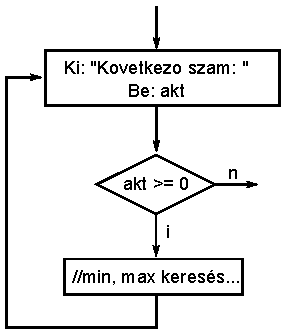
\includegraphics{vesszo.pdf}
    \column{0.6\textwidth}
      Vessző operátor
      \begin{itemize}
        \item összetett, külön-külön is értelmes kifejezésekből álló kifejezés szerepeltethető ott, ahol csak egy kifejezés állhat
        \item a kifejezés értéke az utolsó részkifejezés értéke
      \end{itemize}
  \end{columns}
\end{frame}

%8
\begin{frame}
  Logikai kifejezések
  \begin{itemize}
    \item \texttt{bool} típus
    \item \texttt{false} \kiemel{$\equiv$} 0
    \item \texttt{true} \kiemel{$\equiv$} 1
    \item nulla értékű egész $\to$ hamis
    \item nem nulla értékű egész $\to$ igaz
    \item \texttt{if(db) ...} \kiemel{$\equiv$} \texttt{if(db != 0) ...}
    \item \texttt{if(!db) ...} \kiemel{$\equiv$} \texttt{if(db == 0) ...}
  \end{itemize}
\end{frame}

%9
\section{Hátultesztelő ciklus}
\subsection{Logikai típus és operátorok}
\begin{frame}
  \meret{6}
  \begin{exampleblock}{\textattachfile{haromszog1.cpp}{haromszog1.cpp}}
    \vspace{-.2cm}
    \meret{6}
    \lstinputlisting[style=cpp,numbers=left]{haromszog1.cpp}
    \vspace{-.2cm}
  \end{exampleblock}
\end{frame}

%10
\begin{frame}
  Hátultesztelő ciklus -- a ciklusmag egyszer biztosan lefut
  \begin{columns}[c]
    \column{0.35\textwidth}
      \begin{center}
        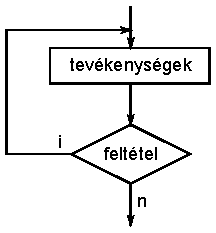
\includegraphics{hatul.pdf}
      \end{center}
    \column{0.6\textwidth}
      do \{ \\
      \hspace{0.5cm} \emph{tevékenységek} \\
      \} while(\emph{feltétel\_kifejezése});
  \end{columns}
\end{frame}

%11
\begin{frame}
  Logikai operátorok
  \begin{itemize}
    \item \kiemel{\texttt{!}}, \kiemel{\texttt{not}}: logikai nem, tagadás
    \item \kiemel{\texttt{||}}, \kiemel{\texttt{or}}: logikai (megengedő) vagy
    \item \kiemel{\texttt{\&\&}}, \kiemel{\texttt{and}}: logikai és
  \end{itemize}
  \vfill
  Igazságtáblázat \\
  \begin{tabular}{lllll}
    a & b & not a & a or b & a and b \\ \hline
    \kiemel{false} & \kiemel{false} & \kiemelZ{true} & \kiemel{false} & \kiemel{false} \\
    \kiemel{false} & \kiemelZ{true} & \kiemelZ{true} & \kiemelZ{true} & \kiemel{false} \\
    \kiemelZ{true} & \kiemel{false} & \kiemel{false} & \kiemelZ{true} & \kiemel{false} \\
    \kiemelZ{true} & \kiemelZ{true} & \kiemel{false} & \kiemelZ{true} & \kiemelZ{true} \\
  \end{tabular}
  \vfill
  (Rész)kifejezések kiértékelésének optimalizálása (short-circuit evaluation)
\end{frame}

%12
\begin{frame}
  \begin{exampleblock}{\textattachfile{haromszog2.cpp}{haromszog2.cpp} -- A feladat átfogalmazása egyszerűsíti a megoldást}
    \vspace{-.2cm}
    \meret{7}
    \lstinputlisting[style=cpp,numbers=left]{haromszog2.cpp}
    \vspace{-.2cm}
  \end{exampleblock}
\end{frame}

%13
\section{Rajzolás a képernyőre}
\subsection{Szimbolikus állandók, összevont és egyoperandusos operátorok}
\begin{frame}
  \begin{exampleblock}{\textattachfile{kor1.cpp}{kor1.cpp}}
    \vspace{-.2cm}
    \scriptsize
    \lstinputlisting[style=cpp,numbers=left]{kor1.cpp}
    \vspace{-.2cm}
  \end{exampleblock}
\end{frame}

%14
\begin{frame}[fragile]
  Problémák:
  \begin{itemize}
    \item a kurzor pozicionálása korlátozott
    \item rengeteg helyen szerepel ugyanaz a konstans: nehézkes módosítás, hibalehetőségek
    \item a karakterek kb. kétszer magasabbak, mint amilyen szélesek
  \end{itemize}
  \begin{block}{Kimenet}
    \vspace{-.3cm}
    \scriptsize
    \begin{verbatim}
     *     
  *******  
 ********* 
 ********* 
 ********* 
***********
 ********* 
 ********* 
 ********* 
  *******  
     *
\end{verbatim}
\vspace{-.3cm}
  \end{block}
\end{frame}

%15
\begin{frame}
  \begin{exampleblock}{\textattachfile{kor2.cpp}{kor2.cpp}}
    \vspace{-.2cm}
    \scriptsize
    \lstinputlisting[style=cpp,numbers=left]{kor2.cpp}
    \vspace{-.2cm}
  \end{exampleblock}
\end{frame}

%16
\begin{frame}[fragile]
  \begin{columns}[c]
    \column{0.6\textwidth}
    \texttt{\#define}
    \begin{itemize}
      \small
      \item szimbolikus állandók, egyszerű makrók
      \item előfeldolgozó ,,egyszerű'' szöveghelyettesítést végez
      \item \kiemel{Nincs pontosvessző a végén!}
    \end{itemize}
    \vfill
    Összevont operátorok
    \begin{itemize}
      \small
      \item \texttt{sor += 2;} \kiemel{$\equiv$} \texttt{sor = sor+2;}
      \item $+$=, $-$=, *=, /=, \%=
    \end{itemize}
    \vfill
    Egyoperandusos $+$ és $-$ operátorok
    \column{0.35\textwidth}
    \begin{block}{Kimenet}
      \vspace{-.3cm}
      \meret{9}
      \begin{verbatim}
            *          
      *************    
    *****************  
   ******************* 
   ******************* 
  *********************
   ******************* 
   ******************* 
    *****************  
      *************    
            *
\end{verbatim}
      \vspace{-.3cm}
    \end{block}
  \end{columns}
\end{frame}

%17
\section{Bolvasás karakterenként}
\subsection{Állapotváltások figyelése, operátorok precedenciája}
\begin{frame}
  \begin{exampleblock}{\textattachfile{szamlalo.cpp}{szamlalo.cpp} -- Betűk, szavak, sorok számlálása}
    \tiny
    \lstinputlisting[style=cpp,numbers=left]{szamlalo.cpp}
  \end{exampleblock}
\end{frame}

%18
\begin{frame}
  Egy karakter beolvasása: \kiemel{\texttt{int get()}}\\
  Karakter ábrázolása \texttt{int} típusban\\
  Bemenet vége: \kiemel{\texttt{EOF}} $\to$ \kiemel{\texttt{<cstdio>}}\\
  Műveleti sorrend! \kiemel{\texttt{while((k=cin.get()) != EOF) \{}}\\
  A \kiemel{\texttt{szoban}} szerepe  
\end{frame}

%19
\begin{frame}
  \begin{center}
    Operátorok precedenciája és asszociativitása
    \vfill
    \scalebox{.8}{%
    \begin{tabular}{ll}
    Operátor & Asszociativitás \\ \hline\hline
    a$++$ a$--$ & balról jobbra \\ \hline
    $++$a $--$a & \multirow{4}{*}{jobbról balra} \\
    $+$a $-$a & \\
    ! & \\
    sizeof & \\ \hline
    a*b a/b a\%b & \multirow{6}{*}{balról jobbra} \\
    a$+$b a$-$b & \\
    < <= > >= & \\
    == != & \\
    \&\& & \\
    || & \\ \hline
    = $+$= $-$= *= /= \%= & jobbról balra\\ \hline
    , & balról jobbra \\ \hline
    \end{tabular}
    }
  \end{center}
\end{frame}

%20
\section{Többirányú elágazás}
\subsection{if \dots else if \dots else \dots}
\begin{frame}
  \begin{columns}[c]
    \column{.55\textwidth}
      \begin{exampleblock}{\textattachfile{ordinal1.cpp}{ordinal1.cpp} -- Angol sorszámnevek}
        \vspace{-.2cm}
        \scriptsize
        \lstinputlisting[style=cpp,numbers=left]{ordinal1.cpp}
        \vspace{-.2cm}
      \end{exampleblock}
    \column{.4\textwidth}
      Problémák: \begin{itemize}
        \item nagyon sok irányú elágazás
        \item felesleges osztások
      \end{itemize}
  \end{columns}
\end{frame}

%21
\subsection{switch}
\begin{frame}
  \begin{exampleblock}{\textattachfile{ordinal2.cpp}{ordinal2.cpp}}
    \vspace{-.2cm}
    \meret{7}
    \lstinputlisting[style=cpp,numbers=left]{ordinal2.cpp}
    \vspace{-.2cm}
  \end{exampleblock}
\end{frame}

%22
\begin{frame}
  \begin{itemize}
    \item \kiemel{switch}(\emph{kifejezés}) \emph{utasítás}
    \item \emph{kifejezés} egész típusú
    \item \emph{utasítás} tartalmazhat
    \begin{itemize}
      \item több \kiemel{case} \emph{konstans-kifejezés: utasítás}-t,
      \item nulla vagy egy \kiemel{default:} \emph{utasítás}-t
    \end{itemize}
    \item végrehajtás leáll:
    \begin{itemize}
      \item \kiemel{switch} blokkjának végén
      \item az első \kiemel{break} utasításnál
    \end{itemize}
    \item \emph{konstans-kifejezés} egész típusú
    \item \emph{kifejezés} és \emph{konstans-kifejezés} értékeinek összehasonlítása
    \item több \kiemel{case} címke is címkézheti ugyanazt az utasítást, de minden 
címkének egyedinek kell lennie
    \item \kiemel{switch} utasítások egymásba ágyazhatóak
  \end{itemize}
\end{frame}

\end{document}
